\chapter{搜索引擎}
现代搜索引擎是一种检索互联网信息的应用程序,主要包括三个模块:采集信息、建立索引、检索信息。搜索引擎是传统信息检索的一个重要应用,它使用计算机程序(网络爬虫或蜘蛛)自动采集互联网数据,然后对采集到的信息进行合理组织与处理(去重、索引等),根据前台搜索界面接收到的用户检索需求,即时迅速地从采集数据中检索到相关文档,并按照相关程度由高到低以列表的形式反馈给用户。搜索引擎肇始于20世纪末的加拿大,经过20多年的迅猛发展,已经成为人们获取信息的一个重要手段。

\ornamento
\section{搜索引擎简史}
1990年,加拿大McGill大学的Alan Emtage、Peter Deutsch与Bill Wheelan联合开发出的一种在线FTP文件索引工具\textbf{Archine},堪称世界首个搜索引擎。它汇集上百个计算机系统的FTP文件资源生成一个文件目录,用户可以使用Unix grep命令查询文件名,从而确定存储目标文件的计算机系统。1992年,Nevada大学的Steven Foster与Fred Barrie出于相同目的开发出\textbf{Veronica},用于搜索普通文本文件。1993年,Utah大学的Rhett Jones与Veronica目标同又开发出\textbf{Jughead}。Veronica与Jughead均受到Archine的影响,分别通过Archine Comic的两个经典漫画人物Veronica Lodge与Jughead Jones向Archine致敬,并且二者发送文件均是基于Gopher系统。

1993年6月,MIT大学的Matthew Gray期望能够追踪互联网发展速度,于是就创造出了世界上第一个网络爬虫程序万维网\textbf{Wanderer},更新以后爬虫程序能够获取真实的网址。爬虫程序每天访问同一个网页上百次,严重影响互联网的速度,人们开始质疑其用处。1993年10月,Martijn Koster开发出\textbf{ALIWEB}(Archie-Like Indexing of the Web)。ALIWEB只抓取少量网页元信息的,允许用户自己提交期望能被索引到的网页数据,如此可以节省大量的带宽资源。对于Wanderer,ALIWEB代表一种强有力的回应,遗憾的是许多人不知如何提交自己的网站。截至1993年12月,陆续又涌现出三个基于网络爬虫的搜索引擎:Scotland的\textbf{JumpStation}、Colorado大学Oliver McBryan的\textbf{万维网蠕虫}、NASA的\textbf{RBSE}(Repository-Based Software Engineering)爬虫。JumpStation采集网页的标题与头部信息,并使用简单的线性搜索执行检索。互联网数目的不断增长最终将JumpStation淘汰出局。万维网蠕虫对网页标题信息及URL建立索引,但是它与JumpStation一样,对检索到的网页一视同仁按照顺序进行排列。RSBE爬虫则实现了一个排序系统,但没有意识到链接分析或者网页内容缓存的重要性。如果用户无法提供确切名称,系统仍然难以找到目标文件。

1993年2月,斯坦福大学六名学生Graham Spencer、Joe Kraus、Mark Van Haren、Ryan Mc Intyre、Ben Lutch和Martin Reinfried成立Architext项目,意图利用字词间关系的统计分析提升搜索效率。1993年6月,他们发布了开发的搜索软件\textbf{Excite}用于网络搜索。1999年1月,@Home以65亿美元的价格收购Excite,并易名为Excite@Home。2001 年10月,Excite@Home破产,InfoSpace以1000万美元的价格将其买下。2002年5月,Excite停止使用自己的搜索引擎,改用元搜索引擎Dogpile。

1994年1月,世界上第一个提供分类目录和搜索功能的\textbf{EINet Galaxy}上线。1994年4月,斯坦福大学博士生Jerry Yang与David Filo共同创办\textbf{Yahoo!}用于收集它们喜欢的网页。随着收录数目与访问量的增加,Yahoo!开始支持简单的数据库搜索。由于Yahoo!收录的网页需要经过手工处理,算不上真正意义的搜索引擎。Yahoo! 陆续采用Altavista、Inktomi、Google提供的搜索引擎服务,推动了搜索引擎技术的发展。1994年4月20日,华盛顿大学的Brian Pinkerton发布
\textbf{WebCrawler},它是世界上第一个支持全文检索的搜索引擎。1994年7月20日,卡内基梅隆大学的Michael Mauldin研发的\textbf{Lycos}正式发布,它是搜索引擎发展史上的一次革命,不仅提供相关性排名,还支持前缀匹配与单词近似匹配,也是第一个在搜索结果页面中实现网页自动摘要,并且它的数据量远超其他搜索搜索引擎。1999年4月,Lycos改由Fast提供搜索引擎服务。1994年底,又一个重要的搜索引擎\textbf{Infoseek}发布。Infoseek友善的用户界面、大量附加服务使它声望日隆。而1995 年12月与Netscape 的战略性协议,使它成为一个强势搜索引擎:当用户点击Netscape浏览器上的搜索按钮时,弹出Infoseek的搜索服务,而此前由Yahoo! 提供该服务。2001 年2 月,Infoseek改用Overture的搜索结果。

1995年,华盛顿大学的Eric Selberg 和 Oren Etzioni开发出\textbf{MetaCrawler},成为世界首个元搜索引擎。元搜索引擎对用户的检索请求进行转换处理,按照格式要求提交给多个成员搜索引擎,最终将所有成员搜索引擎的搜索结果进行汇总并反馈给用户。1995年12月,\textbf{AltaVista}发布亮相,它推陈出新提供大量的创新服务,迅速成为搜索领域的一支新秀。它是第一个支持自然语言搜索、第一个支持高级搜索语法(如AND,OR,NOT 等)、并声称是第一个支持用户自主提交或删除网站网址,并保证24小时内可以检索到的搜索引擎。1995年9月26日,加州伯克利大学的Eric Brewer、Paul Gauthier联合创立\textbf{Inktomi}。1996年5月20 日,Inktomi公司正式成立,并发布新的搜索引擎\textbf{HotBot}。Inktomi公司声称HotBot每天抓取的网页数目超过1000万,远超其它搜索引擎。Hotbot成为随后几年最受欢迎的搜索引擎之一。

1998年9月4日,斯坦福大学的Larry Page与Sergey Brin联合成立\textbf{Google}公司。2004年8月19日,在纳斯达克上市。由于技术先进,经过短短十多年的发展,Google 已经成为全球最大的搜索引擎,搜索服务覆盖全球30多种语言、100多个国家。

1997年,挪威科技大学的Tor Egge成立FAST(Fast Search \& Transfer)公司,1999年5月发布搜索引擎\textbf{AllTheWeb}。FAST试图复制Inktomi的模式,向其他搜索引擎提供数据。它宣称在数据的新颖性、高级搜索功能、搜索结果聚类、本地化显示、图片搜索方面都比Google更具优势。2003年2月,FAST网络搜索部门被Overture 收购。2004年3月25日,Overture被Yahoo!收购。2011年4月4日,alltheweb.com网站重定向到Yahoo!搜索。

2000年,Rutgers大学的Apostolos Gerasoulis及其同事创立\textbf{Teoma},2001年春正式上线。2001年9月11日被Ask Jeeves以大约400万美元的价格收购,为ask.com提供搜索服务。Teoma排名算法ExpertRank比较独特,它同时基于主题分类、链接分析给网页排名。2000年,前Infoseek工程师Matt Wells创立\textbf{Gigablast},索引了2 亿多网页,向合作网站提供大规模高性能的实时信息检索服务。目前,Matt Wells是Gigablast唯一的维护人员,并于2013年7月将代码开源托管到GitHub。2000年5月16日,Yeogirl Yun创立\textbf{WiseNut},并于2001年9月正式上线。WiseNut引进一种新型数据库,并发明一种新技术WiseGuide实现对搜索结果自动聚类,但是对高级搜索、布尔查询、网页快照等功能它却视而不见。2002年4月,被分类目录提供商LookSmart以900万美元的价格收购,试图成为主流搜索引擎。

1997年10月29日,北京大学“网络与分布式系统”研究室研发的“\textbf{天网}”中英文搜索引擎系统正式在CERNET上提供服务。它是国家“九五”重点科技攻关项目“中文编码和分布式中英文信息发现”的研究成果,提供北京大学、中国科院等FTP站点的检索。2000年初,在国家973重点基础研究发展规划项目基金资助下成立“天网”搜索引擎课题组,继续为天网提供技术支持。1998年1月,\textbf{Openfind}创立,并由台湾中正大学吴升教授领导的GAIS实验室提供技术支持。Openfind是当时最好的中文搜索引擎,鼎盛时期同时为三大门户网站新浪、奇摩、雅虎提供中文搜索服务。2002年6月,Openfind重新发布基于GAIS30工程的Openfind搜索引擎Beta版,推出多元排名(PolyRank)算法,宣布累计抓取网页35亿,并踏入英文搜索领域。2000年1月18日,超链分析专利发明人、前Infoseek资深工程师李彦宏(Gigablast的创始人Matt Wells是其在Infoseek的同事)与UC Berkeley大学博士徐勇联合创立\textbf{百度}公司。2000 年6 月,百度正式推出独立搜索门户baidu.com,并开始为多个门户网站(如搜狐、新浪、雅虎中文等)提供搜索服务。2001年10月22日正式发布Baidu搜索引擎。2005 年,百度在美国纳斯达克上市,成为首家进入纳斯达克成分股的中国公司。百度提供了音乐、视频、图片、百科、文库等各种搜索服务,成为目前全球最大的中文搜索引擎。

\section{图像搜索}
目前,许多通用搜索引擎都提供了一种“以图搜图”的图片搜索功能,实现图片搜索的关键技术是“感知哈希算法”(Perceptual Hash Algorithm,PHA),对每张图片生成一个“指纹(Fingerprint)”字符串,利用指纹信息,就可以实现图片相似程度的比较,进而对图片做相似、相关程度的排名。

PHA是一组可以比较的哈希函数,抽取多媒体文件的特征生成哈希值,即便在图片放缩、颜色发生微小改变以后,仍然能够通过相似性比较将其识别出来,对于加密哈希函数(如MD5和SHA1),则可能会产生截然不同的哈希值,无从比较。

利用PHA生成哈希值只需要五个简单步骤:
\begin{enumerate}[(1)]
  \item 缩小尺寸:在图片表示中,使用低频段表示图片的结构,而高频段则用以渲染细节。在图片搜索中,图片的细节部分通常无关紧要,若要将其剔除,最简单快捷的方式是缩小图片的尺寸,比如将图片缩小到$8\times 8$的尺寸,总共64个像素(Pixel,1个像素对应一组三基色RGB),只保留结构、明暗等基本信息,摒弃不同尺寸、比例带来的图片差异。
  \item 简化色彩:将缩小后的图片,转为一个64级灰度(Grayscale)。也就是说,所有像素点总共只有64种颜色。
  \item 计算平均值:计算所有64个像素的灰度平均值。
  \item 比较像素的灰度:将每个像素的灰度,与平均值进行比较。大于或等于平均值,记为1;小于平均值,记为0。
  \item 计算哈希值:将上一步的比较结果组合构成一个64位整数,这就是这张图片的指纹。
\end{enumerate}

在图片生成指纹信息后,可以统计指纹信息中不同位的个数(Hamming距离),比较图片的相似程度,比如不同位的个数小于5就说明两者是相似的。

PHA的优点是简单快速,不受图片大小缩放的影响,缺点是图片的内容不能变更,因为即便是在图片上加几个文字,就无法识别了。所以,它的最佳用途是根据缩略图,找出原图。

实际应用中,往往采用更强大的pHash算法和SIFT算法,它们能够识别图片的变形,只要变形程度不超过25\%,就能匹配原图。这些算法虽然更复杂,但是基本原理相同:先将图片转化成哈希字符串,然后再进行比较。

\subsection{颜色分布法}
颜色分布法(Color Histogram)抽取图片中的主要颜色,并产生颜色直方图。每个像素都是由三基色(RGB)构成,每个基色可以取256个值,那么整个颜色空间共有1600万($256^3$)个颜色。为了降低计算量,将0~255分成四个区:0~63为第0区,64~127为第1区,128~191为第2区,192~255为第3区,则每种基色只需要4个数字(0~3)即可表示,则整个颜色空间仅仅需要64($4^3$)个组合就可以完全表示(如图\ref{fig:colordistribution}),只要取出每个组合的像素统计量就可以生成图片的指纹特征。
\begin{figure}[htbp]
  \centering
  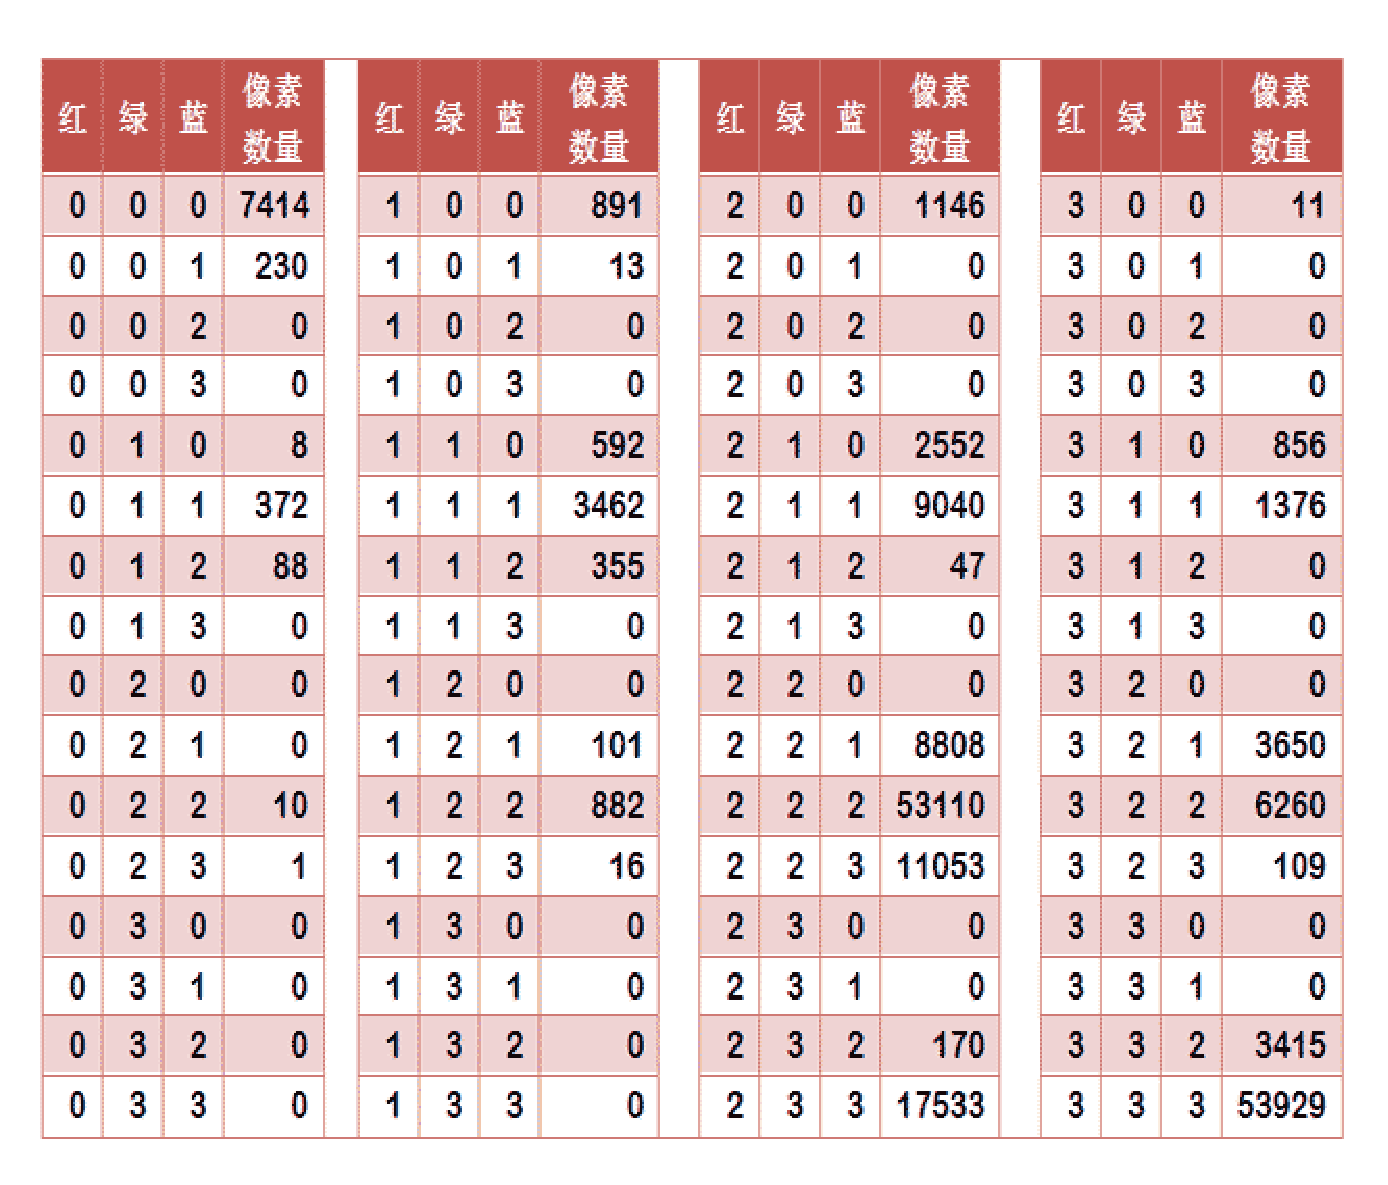
\includegraphics[width=0.95\textwidth]{figures/colordistribution.eps}
  \caption{颜色分布图}\label{fig:colordistribution}
\end{figure}

\subsection{大津阈值法}
图片处理中最常用的方法是将图片转换成较小的灰度图片,比如$50\times 50$,然后,再将灰度图片转成黑白图片(0-黑色,1-白色)。最终,使用0-1矩阵做相似性判断。在图片由灰度图片转换到黑白图片时,阈值选择是一个重要的步骤。

一般地,如果两张图片相似,那么它们的黑白轮廓自然也相近,一个合理的阈值应该能够正确呈现出图片的黑白轮廓,而反映轮廓清晰程度的重要因素是前景色与背景色的反差,反差越大则轮廓越明显。这就意味着,通过最小化前景色和背景色各自的类内差异(Minimizing the Intra-class Variance),或者最大化类间差异(Maximizing the Inter-class Variance)就可以找到理想的阈值$\theta$。

1979年,日本学者大津展之证明“类内差异最小”与“类间差异最大”是等价的,对应相同的阈值,这种通过最优化类内或类间差异,确定最佳阈值的简单方法就是大津阈值法(Otsu's Thresholding Method)。

假定一张图片共有$n$个像素,其中灰度值小于$\theta$的像素有$n_1$个,大于等于$\theta$的像素有$n_2$个,那么由此可以计算两种像素的权值$\omega_1 = n_1/n$和$\omega_2=n_2/n$。

再假定所有灰度值小于$\theta$的像素的平均值和方差分别为$\mu_1$和$\sigma_1$,所有灰度值大于等于阈值的像素的平均值和方差分别为$\mu_2$和$\sigma_2$,那么,可以计算类内差异和类间差异:
\begin{eqnarray}
  V_r &=& \omega_1\sigma_1^2 + \omega_2\sigma_2^2 \\
  V_e &=& \omega_1\omega_2(\sigma_1 - \sigma_2)^2
\end{eqnarray}
可以证明,两个等式是等价的,不过,从计算难度看,后者的计算要容易一些。

有了$50\times 50$像素的黑白缩略图,就等于有了一个$50\times 50$的0-1矩阵。矩阵的每个值对应原图的一个像素,0表示黑色,1表示白色。两个特征矩阵的不同之处越少,说明两张图片越相似。

\subsection{VisualRank}
在2008年北京国际万维网会议上,Google的两名科学家Yushi Jing和Shumeet Baluja介绍了一种图片搜索新型算法VisualRank,它通过直接分析图片内容,并充分利用图片名称、网络链接地址或者其他文本内容,寻找和排列图片。综合了图像识别、相似图像排序技术,应用到大规模图像搜索\cite{jing2008visualrank}。

\section{元搜索引擎}
元搜索引擎(简称“元搜”)是一种“超搜索引擎”。它通过统一的搜索界面,将用户的检索请求,提交给多个搜索引擎,并将各搜索引擎返回的搜索结果经过滤重、聚类、重排等过程,展示给用户(见图\ref{fig:metase})。接收元搜索引擎检索请求的搜索引擎,称作“源搜索引擎”、“成员搜索引擎”或者“独立搜索引擎”,我们在后文统一称之为“独立搜索引擎”。一般而言,元搜没有独立的爬虫,依赖于独立搜索引擎而存在。

\begin{figure}[ht]
  \centering
  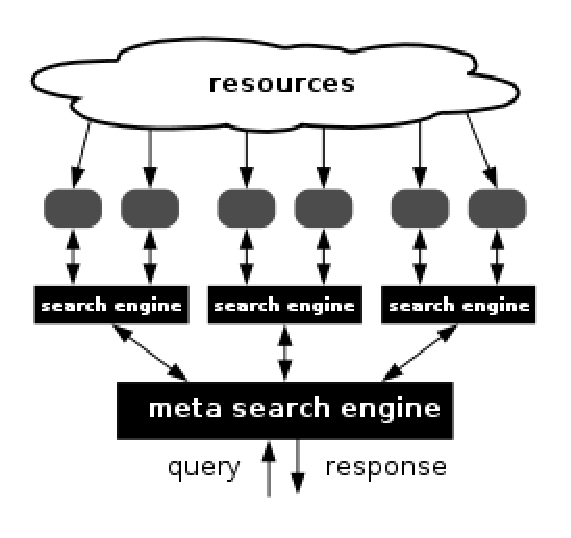
\includegraphics[width=0.5\textwidth,height=5cm]{figures/MetaSE.eps}
  \caption{元搜索引擎工作流程草图}\label{fig:metase}
\end{figure}

国外元搜的发展比国内更成熟,无论界面设计,还是搜索技术都有大量可借鉴之处,这里简单介绍几个比较典型的元搜及其基本功能。

\subsection{Savvy Search}
睿智搜索(Savvy Search)是世界上第一个元搜索引擎,由科罗拉多州立大学研究生Daniel Dreilinger开发,1995年3月正式上线。
睿智搜索运行在五台机器上,三个Sun SpackStation,两个IBM RS 6000s,其设计关注于平衡最大化精度、最小化计算及网络资源消耗两个相互冲突的目标,根据对各个独立搜索引擎长期的观察,确使每次提交给睿智搜索的检索词,依据系统历史统计数据,向最可能返回相关结果的独立搜索引擎提交检索请求,不仅确保精度,还减少了向所有独立搜索引擎提交查询的开销。
睿智搜索是一个并行检索的元搜索引擎,可调用二十一个独立搜索引擎,检索包括WEB、USENET新闻组、软件、参考工具、人、技术报告等信息。每次最多可同时检索五个搜索引擎的数据库,也可以作为独立的搜索引擎使用。它还支持布尔查询,由于并非所有成员搜索引擎都能正确处理布尔操作符,搜索结果可能并不精确。它还允许用户指定每个搜索引擎返回结果的数目,如选择“聚合结果”选项,系统将对结果集作去重处理。默认情况下,它只显示各个独立搜索引擎前二十条命中记录。另外,它还支持包括中文在内的二十三种语言版本的搜索功能。
1999年10月14日,CNet网络集团宣布以2200万美元股票和现金组合的形式将其收购,此时睿智搜索已经融合了三百多个网络搜索引擎的搜索结果,月均使用用户达到百万。

\subsection{Meta Crawler}
1994年,华盛顿大学研究生Eric Selberg和助理教授Oren Etzioni共同开发出Meta Crawler,并在1995年7月发布。Meta Crawler与Savvy搜索同年开发同年发布,人们常误以为它是世界上第一个元搜索引擎。1995年初,Meta Crawler已经运行在四个AlphaStation工作站上,日均处理几万条查询,给华盛顿大学宽带造成巨大的压力。1995 年夏,两人成立NetBot公司进行商业推广,但是由于没有明确的盈利模式,还需要向独立搜索引擎支付查询费用,不得己将使用权转让给Go2Net。2000年,Go2Net与InfoSpace 合并,虽然Meta Crawler仍提供独立的元搜索服务,地位已是今非昔比。
Meta Crawler聚合了Google,Yahoo!,Bing,Ask.com,About.com,MIVA,LookSmart和其他主流搜索引擎的结果,提供网页、图片、视频、新闻的搜索服务。在高级搜索页面,用户可以设置最大等待时长(5秒至2分钟)和每个搜索引擎返回结果的最大数目(10、20、30),对各个独立搜索引擎的结果集成,删除重复的URL和死链接,将排序结果以统一的形式显示给用户。

根据Eric Selberg自己的介绍,他们仅仅使用3到5个月的时间开发完成Meta Crawler,其中最复杂的一块就是网络处理,网络协议、并行I/O上占用了绝大部分时间。在开发时两人完全没有考虑过具体的商业模式,只是在发布后才逐渐摸索出一套商业模式:通过在搜索结果中显示独立搜索引擎的推广广告,实现利润共享。Eric认为,元搜面对的问题有很多,主要包括三点:(1)资源发现,能够自动发现新的搜索引擎并将其加入到独立搜索引擎列表;(2)用户认同,把用户的注意力从独立搜索引擎吸引到元搜;(3)商业模式,很难找到一个让所有独立搜索引擎提供商都满意的商业模式。

\subsection{Dogpile}
1996年,Aaron Flin创立了Dogpile,11月正式投入运营。1999年8月,以价值5500万美元的股票和现金作价卖给Go2Net,使得Go2Net旗下同时拥有了两个最受欢迎的元搜索引擎:Meta Crawler与Dogpile。2000年8月,InfoSpace与Go2Net集团合并,但Meta Crawler和Dogpile继续分开运营。2002年初,InfoSpace又以1,000万美元的低价收购Excite和Web Crawler,以麾下四个最著名的元搜索引擎独霸元搜索市场。

Dogpile聚合了顶级搜索引擎Google、Yahoo!、Bing、Ask.com和About.com的搜索结果,并在2005年4月、2005年7月、2007年4月同匹兹堡大学(Pittsburgh University)、宾夕法尼亚大学(Pennsylvania State University)、昆士兰科技大学(Queensland University of Technology)研究人员合作,使用上万个查询词,估计几个顶级搜索引擎搜索结果的重复率情况。研究发现,主要搜索引擎(包括Google,Yahoo!,Ask,Bing)搜索结果的重复率低于4\%,2007年的研究结果甚至低于1\%,从而以此证明任何单个独立搜索引擎都不能完全满足用户的检索需求,元搜的存在是有价值的,它可以弥补独立搜索引擎覆盖率不足的问题,聚合多个独立搜索引擎的搜索结果,给用户更多相关的结果。

\subsection{Excite}
1994年,斯坦福大学(Stanford University)的Graham Spencer,Joe Kraus,Mark Van Haren,Ryan McIntyre,Ben Lutch和Martin Reinfried共同创立了Excite,提供包括门户、搜索引擎、电子邮箱、即时信息等多种在线服务。1994年7月,国际数据集团(International Data Group)向其投资10万美元用于开发一个在线服务网站,并于1995 年12月正式上线。1996 年1月,George Bell(错失过以75万美元收购Google的良机)以CEO的身份加盟Excite,并主持收购两个搜索引擎Magellan和WebCrawler。
1996年4月4日,Excite首发200万股股票。由于经营不善,1998年3月31日其净损失竟达到近3千万美元,1999年1月19日@Home Network公司以67亿美元的价格将其收购,并组建新公司Excite@Home,融合@Home的高速网络服务和Excite搜索及门户网站,专注于提供个性化的网络内容服务。由于接二连三的商业决策失误,2001年9月13日Excite@Home申请破产保护,期间Iwon.com与InfoSpace联合投中Excite域名和品牌。2001年12月16日,Iwon.com启用新的Excite门户,并更名为Excite网络公司,继续经营Excite、iWon和另一个门户MyWay。InfoSpace则拥有和运营Excite的网络搜索部分。
2004年3月Ask Jeeves(如今的Ask.com)将Excite网络公司收购,并在2005年,与InfoSpace就美国区Excite业务达成和解,双方共同承担市场成本、共享Excite 搜索业务的利润。

\subsection{Web Crawler}
1994年4月20日,由华盛顿大学(Washington Uiversity)学生Brian Pinkerton开发的Web Crawler发布上线,成为世界上第一个提供全文搜索的网络搜索引擎。1995 年6月1 日,美国在线将其收购,又在1997年4月1日转手卖给Excite,2001年Excite@Home破产后又将其出售给InfoSpace。最初,Web Crawler拥有独立的抓取程序和网页数据库,其主要收入来源于搜索结果页面投放的广告费,在并入InfoSpace以后,作为元搜索引擎向用户提供搜索服务。

\subsection{Vivisimo}


\subsection{Ixquick}
Ixquick是David Bodnick于1998年研发并推出的一个元搜索引擎,自称是全球最大中介搜索引擎,目前支持14个搜索引擎的搜索结果。2000年,Ixquick被一家荷兰公司Surfboard Holding B.V收购。Ixquick背后的独立搜索引擎包括:Teoma,EntireWeb,All the Web,Ask,Bing,Cuil,Exalead,Gigablast,Lycos,AltaVista,WiseNut,LookSmart,Netscape,Open Directory, Qkport, Wikipedia,Statesman,Yahoo与Blekko,不含Google。

2006年6月27日,Ixquick声明删除用户详细浏览信息,并保证在48小时内清除提交搜索的用户IP地址和其他个人信息。2009年1月28日宣布完全停止对用户IP地址的记录。
截止2010年1月,Ixquick已经处理了12亿次查询请求。根据Ixquick公司背景介绍,它是世界上隐私保护做得最好的搜索引擎公司,从2006年起,开始专注对用户隐私的保护,做到不记录用户IP地址、cookies,不搜集而且不与第三方分享用户个人数据,提供安全的、加密的HTTPS/SSL连接。

Ixquick直言提供相似搜索服务的搜索引擎,包括Google、Yahoo!和Bing,以及元搜索市场上,拥有三家马车的InfoSpace是其主要竞争对手。它目前还未上市,在过去的5年里(2006年起)一直都是盈利的,资金充裕,其盈利模式并无特别之处,在搜索结果页面显示相关的“赞助结果”,按照点击次数向广告客户收取费用,但每页显示的“赞助结果”不超过3条,而且全部放到搜索结果的首尾两端。

由于Ixquick难以记忆和拼写,该公司于2009年启用新的域名Startpage\footnote{See http://www.startpage.com/}。有消息称,Ixquick 正在开发邮件服务系统。
\subsection{Mamma}
1996年,由加拿大人Herman Tumurcuoglu开发的网站Mamma.com
\footnote{\href{http://www.mamma.com/}{http://www.mamma.com/}}
正式发布上线。2005年12月22日,Mamma.com以1590万美元收购一家搜索技术公司Copernic,并发行238万股股票。Mamma.com 能够有效整合多个顶级搜索引擎的搜索结果,赢得“搜索引擎之母”的称号。它支持常用检索语法在不同搜索引擎之间的转换,还提供通过Email订制搜索结果的特色服务。Mamma.com还是一个广告网络公司,通过在线推介创收。

\subsection{Kartoo}
2002年04月25日,Laurent Baleydier和Nicholas Baleydier两兄弟联合开发的Kartoo\footnote{See http://www.kartoo.com/}上线,它是一个可视化元搜索引擎,以图形界面的形式展示搜索结果,通过关键词建立语义连接,将搜索结果生成一个聚类图,方便用户选择、缩小搜索范围。2010年1月,由于不明原因关闭。

Kartoo使用的可视化技术是Laurent团队研究三年的成果,使用球形结点代替搜索结果条目,并通过球形节点的大小反映页面的重要程度。Kartoo最引人注目的地方在结点间的语义连接,如果搜索条目之间存在连接,则使用语义关键词标示节点之间的连线。Kartoo易于使用,并且富有趣味性,代价就是加载过慢。

与国际市场形成鲜明对比,国内元搜市场鲜见成功的案例。我们下面介绍国内几个昙花一现的元搜:
\subsubsection{比比猫}
2005年1月1日,新加坡人朱明谦(Kim Choo)和李昌日联合创立了比比猫(Bbmao),并在2006年02月发布上线,它是中国第一家聚类元搜索引擎,通过聚类技术和个人网络收藏夹改善搜索结果。

朱明谦对中国市场的分析可以归纳为以下几点:(1)中国搜索引擎市场差异化程度比较低,元搜的机会比较大。传统搜索引擎公司在底层搜索技术投入巨大,Bbmao 则更注重以上层的数据处理技术、智能搜索技术求生存。(2)大多数元搜没有核心技术,仅仅是整合其他搜索引擎的结果。只要有核心技术,公司就一定有价值,而Bbmao的核心技术就是聚类技术。(3)与独立搜索引擎合作共赢,独立搜索引擎提供搜索结果和竞价排名广告,元搜借着竞价排名广告收入分成。在06年,Bbmao的首席财务执行官Bill Milewski透露,Bbmao的盈利主要靠广告,并协议和Google等各大搜索引擎对广告利润分成。Bbmao期望成为一个社会化搜索引擎网站,其根本是发挥Web 2.0的内核——个人应用,靠用户改善搜索结果,就像Google通过搜索结果的点击改善排名。其特点可以归结为以下几点:
\begin{itemize}
  \item 资源聚合:同时提供Google,百度,雅虎,搜狗和爱问五大搜索引擎组合搜索或单个搜索结果,搜索结果排名是根据网页在各个搜索引擎中结果中出现的次数及排名来确定的,并明确标示各条结果在相应搜索引擎中的排名信息;
  \item 聚类:在搜索结果页面左侧,呈现聚类列表,由用户点击选择目标类别,优化查询结果;
  \item 去重:采用公司开发的FeatureMatch技术;
  \item 快照:提供搜索结果预览;
  \item 网络搜藏夹:注册用户享有的服务,方便用户收藏和共享,期望借此跟踪用户习惯,更好地为用户提供聚类结果,打造社会化搜索圈。
  \item RenqiScore:使用人气得分技术向用户推荐高品质的相关会员,建立属于用户自己的交际网,还可以通过邀请朋友扩大交际圈。
\end{itemize}

2005年,Myspace创始人Brad Greenspan完成对Bbmao的注资,成为BroadWebAsia(BWA)集团在中国的第一笔投资。2006年3月,Bbmao的流量达到每天2万至3万,8月份超过7 万。Bbmao创建以后赢得的诸多赞誉,它启动“比比猫公益搜索”平台,以期打造互联网企业社会责任新方向。目前,Bbmao已经倒闭。Bbmao倒闭的原因有(1)用户习惯:它无法扭转已经习惯使用百度和Google的用户习惯。(2)它只是进行了非经营性网站的备案,并未获得经营性网站信息许可证,不能从事盈利性商业活动。(3)盈利模式单一:它主要与合作伙伴间的点击付费分成。

\subsubsection{万纬}
由上海万纬信息技术有限公司在1999年12月推出,是中国第一个元搜索引擎,集成了包括Google,Yahoo!,HotBot,AltaVista等8个英文搜索引擎,中文雅虎,搜狐、新浪、中文Excite、中文Google等12个中文搜索引擎,起正式版本2002年发布,功能比较完善。

万纬搜索提供的高级搜索功能包括:(1)允许布尔查询,支持AND/OR;(2)结果排列方式有四种选择,包括相关度、时间、网站分类、引擎;(3)选择最大等待结果的时间,7秒到1分钟,默认20秒。(4)允许设置显示的查询结果个数,10到200个,默认为20个。遗憾地是,万纬在2007年7月份就已经停止查询服务。

\subsubsection{搜乐}
搜乐是广州明智科技有限公司推出的一个元搜索引擎。目前,搜乐整合了Google、百度、必应、搜狗、有道、搜搜和中搜等搜索引擎的搜索信息,并支持自动去重。
主页功能显示,搜乐支持对网页、图片、视频、文档、新闻和微博的搜索,其中文档搜索包含的格式有Doc、XLS、PPT、PDF、RTF和TXT。

在“设置”中可由用户指定(1)界面语言,包括中文繁体和简体。(2)搜索语言可不限。(3)每页显示结果3到100条。(4)是否在结果页中显示“推广”项;(5)是否允许在结果页中显示“赞助链接”。

高级选项模仿了部分Google高级搜索的设置,添加对关键词出现位置的设定,包括文档的任何地方、仅标题、仅正文、仅URL和指向文档的链接。此外,它还支持对单个网站的搜索。目前搜乐不支持任何搜索,只有图片和视频展示页面。根据58同城招聘信息,明智科技正在招聘.NET软件工程师(2012年4月11日)和网站美工(2012 年3月21 日),组建创业团队。该公司主营产品是蓝月亮VOD点播系统。

\subsubsection{名捕}
名捕根据搜索类别,提供不同的资源列表方便用户选择,见下表:
\begin{table}[htbp]
\centering
\begin{tabular}{|c|c|}
    \hline\hline
    搜索类别 & 资源网站列表\\
    \hline
    网页 & 百度、搜搜、搜狗、有道、中搜、必应、雅虎、谷歌、即刻\\
    图片 & 雅虎、新浪、必应、搜狗\\
    音乐 & 新浪、搜狗、雅虎、狗狗、搜搜\\
    视频 & 新浪、土豆、优酷、搜搜、搜狗、谷歌、乐视\\
    软件 & 天空、Enet、华军、百度、ZOL、Pchome、新浪\\
    新闻 & 谷歌、有道、搜搜、必应、百度、搜狗\\
    知识 & 知道、雅虎、百科、搜搜、搜狗\\
    博客 & 搜搜、百度、有道、爱问、奇虎、搜狗、谷歌\\
    论坛 & 谷歌、中搜、奇虎、贴吧、搜搜\\
    词典 & 搜搜、爱词霸、海词、有道、沪江、词酷\\
    财经 & 和讯、金融界、谷歌、搜牛、中金\\
    购物 & 谷歌、有道、淘宝、当当、卓越\\
  \hline
\end{tabular}
\end{table}

它只提供搜索引擎的切换,不提供结果排名聚合。从根本上来讲,它只提供了针对各个搜索类别比较权威的站点,供用户挑选。此外,名捕还在首页提供了几个不错的资源——搜索大全、儿歌大全、晨曦五笔、绝妙好词。

\subsubsection{P搜}
P搜是刘洪照历经四年研发的成果,它聚合了百度、Google、Yahoo!、搜狗、有道、搜搜和必应的搜索结果,经过去重,重排,缩小搜索范围,精确查找信息。
根据其本人介绍,第一版搜鸿元搜索引擎(sohong.cn)由于技术瓶颈问题,一直没突破速度限制,搜索耗时略长。在2009年4月份他重写搜鸿,突破了技术瓶颈,并陆续添加竞价排名和后台管理模块,并易名为新牛元搜索(ccniu.com)。后受到115聚合搜索的影响,历时一周对新牛改写,实现了各个模块的松耦合,并通过API整合各个模块,

2009年9月升级到第二版。2010年初新牛上线,放弃服务端处理模式,改用Ajax模式,速度比以前要慢,但节省服务器开支,由于没有独立服务器,Ajax版本超过两秒,原服务端处理在1秒以内。至2011年2月,历经5次代码重写,多次更新,新牛算法趋于合理,搜索结果排序更加人性化。2011年5月8日改版并易名为P搜,采用镜像psou.cn。

\subsubsection{马虎聚搜}
马虎聚搜是BroadWebAsia(BWA)集团在中国投资的第一家互联网公司,提供基于搜索引擎的多种互联网服务。马虎聚搜声称经过技术测试,国内通用搜索引擎在搜索结果前两页当中,重复率约占5-16\%。该公司拥有独特的FeatureMatch技术,可以大幅减少搜索结果中的重复信息。(FeatureMatch——Bbmao)

搜索发现,基本上和百度的搜索结果一样,不同之处在于马虎聚搜会过滤掉百度文库、百度翻译、能够提供直接下载的搜索结果条目,并在每个搜索结果条目前加注序号。如切换到独立搜索引擎,会自动弹出对应的搜索引擎搜索结果页面,若切换到Google、Bing,还会出现中文乱码。支持收藏和预览功能,但最多返回10页搜索结果。对音乐、图片、视频的搜索直接跳转到百度的搜索页面。

\subsubsection{佐意}
佐意网的前身是一佐网络,始建于1998年3月,2007年3月正式更名为佐意网,并启用新域名。佐意是一个集成搜索引擎,提供网页,新闻,软件,游戏,动画,音乐,影视,地图等信息的搜索,能够自动屏蔽掉色情木马不良网站,减少用户的烦恼。2010年10月11日,佐意网终止搜索服务,转为一个以BLOG为主,并提供相关查询的综合性网站。2011年7月1日,佐意官网宣布停止运营,终止所有服务。

\subsubsection{Juxit}
Juxit是Reuben Boyd 于2004年创建和发布的,声称是第一个聚合了中英双语的元搜索引擎。它聚合了Google中文,Yahoo中文,百度,搜狗,MSN,Wisenut 和 Looksmart的搜索结果。Juxit包含购物、旅行、新闻、图片、视频和音频搜索,并提供预览功能。它支持免费的、按点击次数收费的广告,并推出联盟计划(affiliate program),向广告客户支付转介佣金。此外,它还允许广告穿插到搜索结果中。目前,Juxit已经停止运营。

目前中国国内还出现过很多其他元搜,我们将它们全部收录于表~\ref{tbl:cnmetase}。
\begin{table}[htbp]
\centering
\caption{中国元搜索引擎目录}\label{tbl:cnmetase}
\begin{tabular}{|l|l|l|l|l|}
    \hline\hline
    名称 & 介绍 & 发布时间 & 状态\\
    \hline
    \href{http://www.bioon.com/multisearch.htm/}{生物谷} &  张发宝开发,搜索时同时展开多个页面 & 2001年10月 & 正常\\
    \hline
    \href{http://www.suotianxia.com}{索天下} &  -- & 2006年12月14日 & 关闭\\
    \hline
        &  华南师范大学附属中学的叶古于2003年开发,采用CooRank & & \\
    \href{http://coo.hsfz.net/fish/}{MetaFisher} & 自动分网页评级系统优化排序,CooWord2Beta关键词 & 2003年 & 关闭\\
        & 析归纳算法增加搜索深度和广度,CooSimil滤重 & & \\
     \hline
        & 提供了Google+百度,Google+Yahoo!,Google+Yahoo! & & \\
    \href{http://www.xisoso.com/}{Xisoso} &  三种组合的搜索结果,搜索结果还提供del.icio.us  & -- & 关闭 \\
        & 标签和天天网摘(365Key),还支持自动聚类功能 & & \\
    \hline
    \href{http://www.baidugoo.com/}{Baidugoo} &  -- & -- & 关闭\\
    \hline
    \href{http://www.bydou.com/}{北斗搜索} &  深入搜索、相关搜索、可评价结果 & -- & 关闭 \\
    \hline
    \href{http://www.ejear.com/}{壹家搜} &  聚合百度、Google中文、Yahoo!中文的搜索 & & \\
        & 结果,据称对相似结果的处理有其特色 & 2005年11月 & 正常\\
    \hline
    \href{http://www.bbmao.com/}{比比猫} &  聚类、在线收藏共享 & -- & 关闭\\
    \hline
    \href{http://www.hensou.com/}{狠搜} &  -- & -- & 关闭\\
    \hline
    \href{http://www.kwindsoft.com/k-metasearch/}{K风元搜索} &  聚合、收藏功能 & 2007年01月02日 & 关闭\\
    \hline
    \href{http://cn.xooda.com/}{Xooda中国} &  支持16个国家和地区的搜索,而中文支持Google、&&\\
        & 百度、中文雅虎、爱问、搜狗等10多个搜索引擎 & 2007年02月16日 & 关闭\\
    \hline
    \href{http://www.seekle.cn/}{Seekle} &  聚合百度、Google、搜狗、Yahoo!的搜索结果 & 2007年12月30日 & 关闭\\
    \hline
    \href{http://www.pifa.us/}{PIFA} &  -- & 2008年01月13日 & 关闭\\
    \hline
    \href{http://www.sohong.cn/}{搜鸿元搜索} &  艺鸿开发,后易名为搜牛、P搜,支持去重、 &&\\
        & 重排、预览、收藏等功能,使用方便快捷 & 2008年02月19日 & 正常\\
    \hline
        & 基于Ajax技术,聚合谷歌、百度、雅虎、&&\\
    \href{http://www.metasoo.cn/}{觅搜} & 一搜、搜狗、有道等搜索引擎搜索结果 & -- & 正常\\
        & 允许用户自行设置各搜索引擎权重 & & \\
    \hline
    \href{http://www.deyeb.com/}{Deyeb} &  董一萌开发的社会化元搜 & -- & 关闭\\
    \hline
    \href{http://www.soseen.com/}{搜星} &  聚合百度、搜狐、新浪、Google等搜索引擎,可搜索精选网址 & -- & 关闭\\
    \hline
    \href{http://www.1qiso.com/}{一起搜} &  自称全球最大中文元搜,聚合12个中外搜索引擎结果 & -- & 关闭\\
    \hline
    \href{http://www.jopee.cn/}{Jopee} &  聚合百度、Google、搜狗、必应、有道、Ask,简单切换 & -- & 正常\\
    \hline
        & 聚合百度、Google、搜狗、雅虎和中搜,提供网页、 & &\\
    \href{http://www.someta.com/}{搜魅} & 资讯、图片、网站查询,宣称是最优秀的中文元搜索 & 2009年 & 正常\\
        & “搜魅聚合”等于是百度搜索 & & \\
%    \hline
%    \href{http://www.mangken.com/}{芒肯} &  -- & -- & 关闭\\
%    \hline
%    \href{http://www.souk.cn/}{搜客} &  -- & -- & 关闭\\
%    \hline
%    \href{http://www.yok.com/}{YOK} &  -- & -- & 关闭\\
%    \hline
%    \href{http://www.souk.cn/}{搜客} &  -- & -- & 关闭\\
%    \hline
%    \href{http://www.koooi.com/}{酷爱} &  -- & -- & 关闭\\
  \hline
\end{tabular}
\end{table}

\subsubsection{市场层面}
从用户使用的习惯来看,中国大多用户已经习惯使用单个搜索引擎比如百度、Google,查询所需信息。目前,由于Google退出中国市场,将服务器移到香港,但时断时续的状态导致用户分流,这就部分造就了如今百度一家独大的局面。

根据iResearc的统计数据,2012年2月Google全球搜索引擎市场份额从1月份的75.9\%下降到72.1\%,同时Yahoo!的市场份额则从11.1\%上升到16.5\%。即便真如Google前CEO Eric Smith所言,称Google实际市场份额是包含了一部分垂直搜索引擎市场的份额的,但Google行业龙头老大的地位短时期内是无法撼动的。

从易观国际在2011年第四季度的数据可以看到,百度在中国搜索引擎市场上的份额达到78.3\%,而处于第二位的Google则只有16.7\%,搜狗、搜搜等其他搜索引擎的市场份额之和只有5\%。这种格局同iResearch全球搜索引擎市场格局颇为相似,即一家独大,在中国,百度处于绝对垄断地位。相对PC机搜索市场而言,中国无线搜索市场分布则比较均匀,但百度的份额仍然是最大的一块。

iResearch在2011年底预计中国搜索引擎市场规模到2013年将达到438亿元人民币,而根据易观国际在2010年的预测,到2013年市场规模将达到313亿元人民币,虽然二者相差将近100亿,但从整体趋势来看,搜索市场增长的潜力是巨大。

在这个巨头环立的市场中,元搜要想生存、获得一席之地,首先要有有明确的用户群和市场定位,推崇用户体验至上;其次,由于元搜会分走独立搜索引擎的部分流量,影响其广告业务,应努力寻找同独立搜索引擎合作的结合点,尽可能营造计较有利的发展环境,打消独立搜索引擎对元搜的戒心,避免成为众矢之的。如2008年4 月7日,李彦宏到上海交大演讲。在互动时有学生提到使用“百Google度”同时搜索百度和Google,李彦宏称“元搜索没有生命力”,然而给出的理由却很牵强,“元搜索可以同时查询多个搜索引擎的站点,但用户不需要那么复杂的结果,而且相当多的人习惯了用百度”,并奉劝创业者不要往视频搜索上“撞”。

\subsubsection{技术层面(智能选择、去重、聚类、推荐、重排)}
市场再大,没有核心技术的互联网公司终究无法在这个市场立足,元搜更需要核心技术的支撑。通过分析,国内元搜基本可以归为两种模式:
\begin{itemize}
  \item 框架调用:为用户提供在不同搜索引擎之间进行快速切换,基本无核心技术,容易复制;实际上也不能归为元搜的范畴,没有什么参考价值。
  \item 聚合调用(直接抓取或API调用)——用户一次提交,系统把多个独立搜索引擎搜索结果,经过滤重、重排等处理,返回更为合理的聚合结果。其中,虑重、重排等技术是核心,难以复制。
\end{itemize}
第2种模式被普遍认可,它主要存在以下几个问题:
\begin{itemize}
  \item 比使用单个独立搜索引擎查询所需时间更长
  \item 处理高级检索时,需要将检索语句转换为不同独立搜索引擎的标准格式,转换效果不佳并影响到搜索的效率
  \item 搜索结果依赖于独立搜索引擎数据库的大小、数据的质量
  \item 只能从独立搜索引擎数据库中获取搜索结果的有限信息,如排名、摘要信息等,影响搜索结果排名的可信性
  \item 由于部分独立搜索引擎的盈利模式的特殊性,导致其搜索结果中出现竞价排名的商业广告,智能识别出其中的“赞助广告”是一个不小的挑战。识别出不相关的结果页面,如包含木马病毒、色情信息的网页或网站对于改善用户体验是十分重要的,而实现这一目标难度不小
  \item 由于不同搜索引擎对搜索结果的显示格式也是不同的,以一种统一的方式聚合异构的搜索结果展示给用户,处理起来比较复杂,也是影响搜索效率的又一个障碍
  \item 元搜经常需要批量访问独立搜索引擎的数据库,但由于各主流搜索引擎对访问都设置了上限,信息的查全率会受到很大影响
  \item 随着访问量的增加,服务器端流量、数据处理的压力明显增加,因此硬件要求颇高
\end{itemize}
元搜是为弥补传统搜索引擎的不足而出现的一种辅助搜索工具。因此,必须从数据库选择、查询分派、文本选择、虑重、结果聚合、排名和显示等环节寻求突破,而且这些也是未来元搜研究的重点。

\subsubsection{法律层面}
由于元搜没有独立的数据库,需要在用户提交查询以后,选择并抓取独立搜索引擎的数据库。显然,元搜受制于人,可能会由于频繁抓取独立搜索引擎的数据库,影响独立搜索引擎正常服务,或增加其服务成本而面临诉讼风险。这是否又是一桩“只需州官放火,不许百姓点灯”的经典案例呢?具体的互联网数据信息的访问是否受限,可查询相关法规。

\subsubsection{国内环境的特殊性}
在中国搜索市场上,曾经出现过很多元搜索引擎,有些还很优秀,比如Bbmao、万纬,但后来由于不明原因陆续倒闭。其他类型的元搜多是单人开发,核心技术几乎为零,从界面设计到服务性能都与国外成熟的元搜相差甚远,甚至还有一些打着元搜的旗号,使用小偷程序,安装恶意软件,给用户留下很差的印象。因此,若要在中国推出元搜,让更多用户了解元搜的角色和价值、依赖单个搜索引擎的局限性、遗漏重要信息的代价、重拾用户对元搜的信心是首先要做的工作。

另一方面,由于国内对知识产权保护不力,产品一经推出会即刻产生一批跟风者,这种良莠不齐的混乱状况,会给产品形象带来很大的冲击。因此,产品一定要有特色,并有明确的目标受众,能够明显区别于其他类似产品。由于国内众多企业道德问题饱受公众质疑,因此一个坚决抵制不良信息,努力呈现高品质内容,尽力追求企业良知的搜索引擎公司一定是大众所渴望的,也一定可以走得更远。

\subsubsection{商业模式}
在早期,搜索引擎多作为技术提供商,通过为其他网站提供搜索服务收取服务费。2001年,互联网泡沫破灭后,多转向竞价排名的方式。现在主流搜索引擎商业模式(Google的AdWords、百度的竞价排名)由是Bill Gross提出的,“在搜索结果页面显示广告,根据用户点击向广告客户收费”。该模式有两个特点:一是点击付费(Pay Per Click,简称PPC),用户不点击则广告客户不用付费;二是竞价排名,根据广告客户的付费多少给结果排名。

2003年6月,Google推出一种免费的广告计划AdSense,它是一种面向站长的广告服务。网站发布者为访客提供Google网页和网站搜索功能,借由在搜索结果页面投放Google 广告以获取收益。目前,各大搜索引擎已经开始使用这种模式。

元搜依赖独立搜索引擎而存在,从搜索业务的角度来看,元搜与独立搜索引擎是竞争关系。由于市场份额多被少数独立搜索引擎瓜分殆尽,元搜要在这种不对等的关系中生存和发展,必须提出一种既不会伤及独立搜索引擎利益,又能够持续提供搜索业务的方案,即与独立搜索引擎合作。元搜同独立搜索引擎该如何合作,国外元搜市场比较成功的商业模式,比如InfoSpace 公司可以为我们提供一些借鉴。

InfoSpace公司通过旗下的三个元搜索引擎——Dogpile, WebCrawler, MetaCrawler向用户提供搜索服务,是一个上市公司,因此需要按规定定期发布公司相关信息。
2012年3月9日,InfoSpace发布报告,在Business小节中披露,Google, Yahoo!, Bing和其他搜索引擎被InfoSpace称作内容提供商(Content Providers),并且如果部分内容提供商,如Google,Yahoo!向其支付内容发布的费用,则称它们为搜索客户(Search Customer)。

在Search Revenue Source一节中有记录,其主要收入来自内容提供商向其搜索服务中投放的付费广告。广告客户根据用户点击向独立搜索引擎支付费用,InfoSpace 则从中提成。报告中还披露,在2010年和2011年,Google和Yahoo!两家公司占其全部收入来源95\%以上,而其中Google占绝大部分。报告坦言,如若这两家公司减少面向InfoSpace 的业务,或者对之前协议的价格产生异议的话,必然会对InfoSpace的业务和财务构成造成巨大冲击。

%\section{Academic Search Engine}
%\section{Shopping Search Engine}

\section{网页爬虫}
\textbf{网页爬虫}(Crawler),也称\textbf{网络蜘蛛}(Spider)是人工编写的计算机程序,根据预先设计的参数和爬取方式,从互联网上自动下载的网页、图片、音频等各种类型的数据,是搜索引擎的一个重要组成部分。一般地,网页爬虫首先从给定的一组URL列表开始抓取,下载网页并抽取其中的新链接,放置到未访问列表中,接着新一轮爬取,直到遍历全部URL列表为止。

Google、AltaVista、Bing、百度等搜索引擎是面向所有用户的搜索服务,称为\textbf{通用搜索引擎}(General Search Engine)。通用搜索引擎如同一个万花筒,通过释放通用型的爬虫程序,在互联网上漫游,爬取任何可以下载到的网页内容。通用搜索引擎最大的特点是追求覆盖面,所以就出现了早期各个顶级搜索引擎相互比拼索引的网页数量。尽管搜索技术从诞生至今已经发生了天翻地覆的变化,随着社交网络和用户生产的各种私人数据的爆炸式增长,爬取整个互联网并建立索引的追求逐渐脱离现实。因为,用户的需求已经随着数据量的指数增长发生的巨大的变化,细化分割的市场逐渐走上历史的舞台,这就是\textbf{垂直搜索引擎}诞生的基础,也是\textbf{主题爬虫}(Focused Crawler)赖以生存发展的机遇。主题爬虫通过判断访问页面同主题的相关程度有选择的爬取,从而实现以最短的时间开销抓取到最多高质量的相关网页内容。
